\documentclass{article}

\input{C:/Code/TexStudio/templates/structure.tex} % Include the file specifying the document structure and custom commands

%----------------------------------------------------------------------------------------
%	ASSIGNMENT INFORMATION
%----------------------------------------------------------------------------------------

\title{Assignment \#6} 
% Title of the assignment

\author{Name:Cao Mingming \indent \indent ID:2018311770\\ \texttt{cmm18@mails.tsinghua.edu.cn}} 
% Author name and email address

\date{Tsinghua University --- \today} 
% University, school and/or department name(s) and a date


\begin{document}
	\maketitle % Print the title


\section{Problem 2}
 Calculate the transmission of the electric field and intensity for a cavity having mirrors with reflectivity $r_1 \quad r_2$ (and transmission $t_1 \quad t_2$), separation d and con-
taining a medium with transmission t. This is just the case not discussed in the text.

\section*{Solution}
From the bookmwe can draw a figure as following which indicate the how to calculate of transmission.
\begin{figure}[htb]
	\centering
	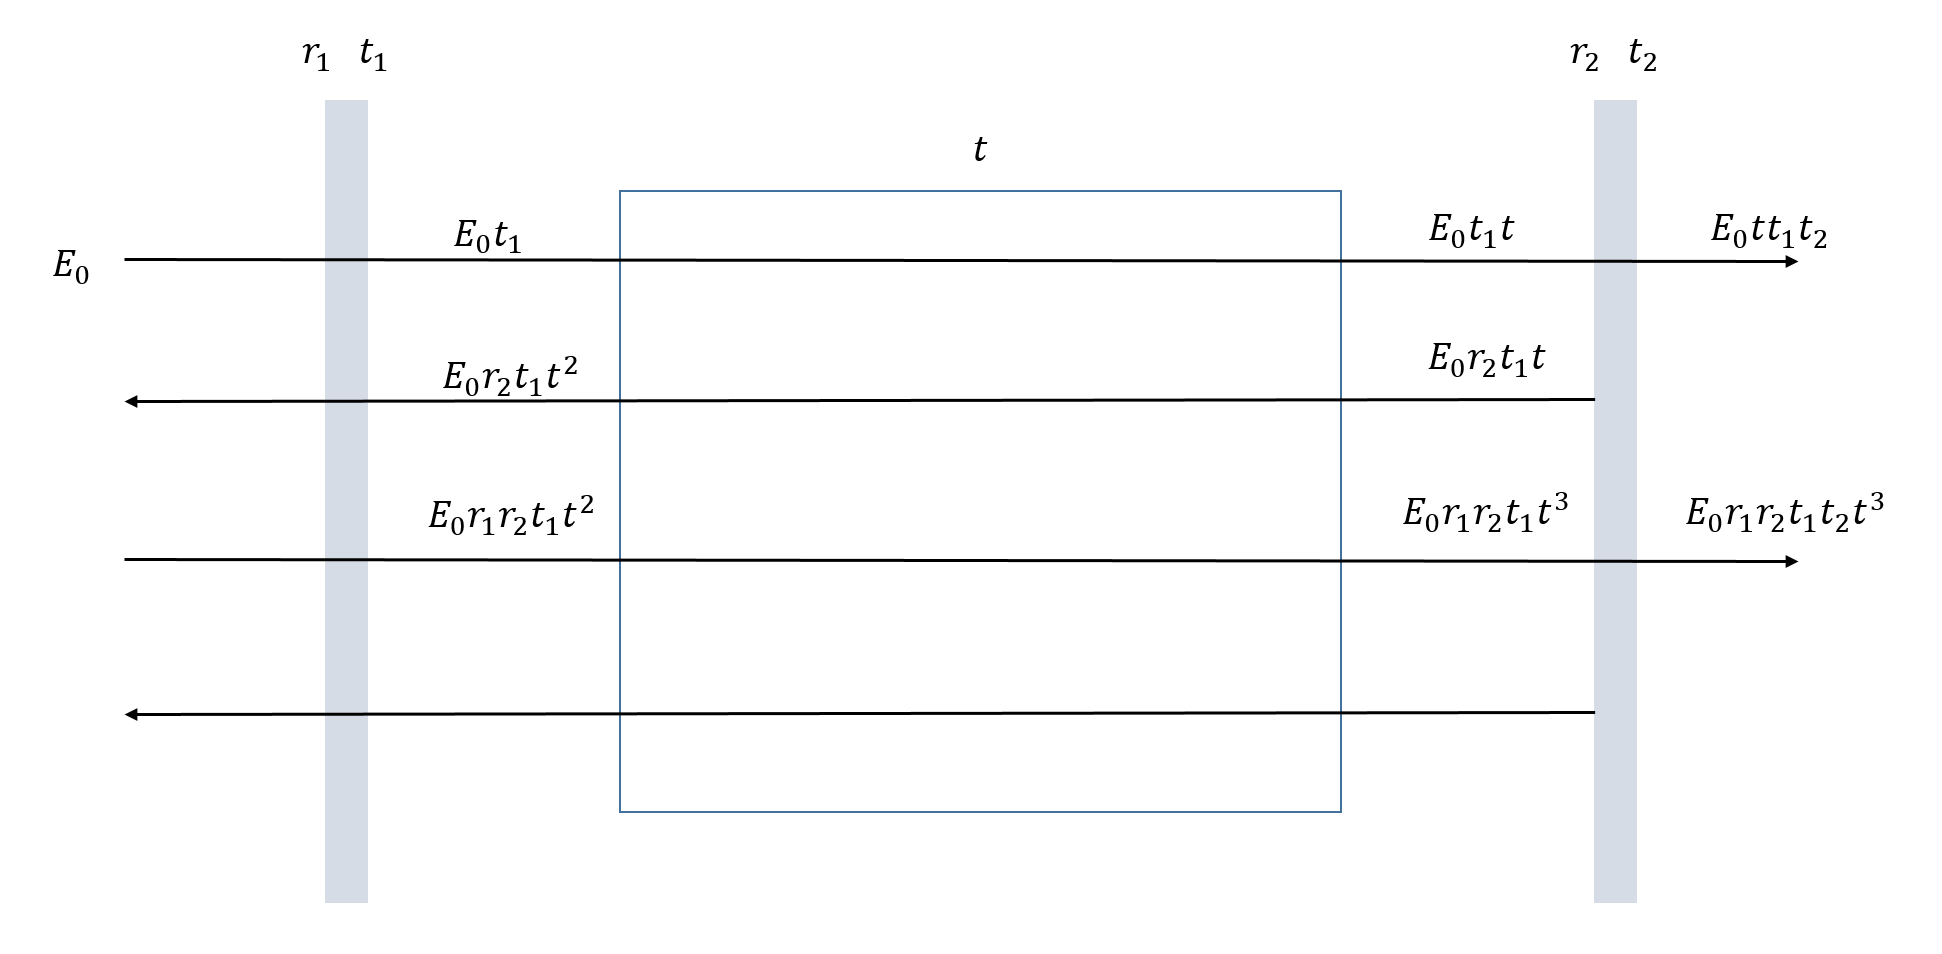
\includegraphics[width=0.8\linewidth]{f2}
	\caption{Transmission Figure}
	\label{fig:f2}
\end{figure}
Therefore we can get,
	\begin{equation}\label{key}
		\begin{aligned}
		E_t&=E_0tt_1t_2(1+q+q^2+...)\\
		&=\frac{E_0tt_1t_2}{1-r_1R_2E^{-I\delta}}
		\end{aligned}
	\end{equation}
where $q=r_1r_2t^2e^{-i\delta}$, and we can calculate the transmission intensity as,
\begin{equation}\label{key}
	\begin{aligned}
		I_t&=|E_t\//E_0|^2\\
		&=I_0\frac{t^2t_1^2t_2^2}{(1-r_1r_2t^2)^2+4r_1r_2sin^2(\frac{\delta}{2})}
	\end{aligned}
\end{equation}
\end{document}

